\documentclass{article}
\usepackage[utf8]{inputenc}
\usepackage{listings}
\usepackage{hyperref}
\usepackage{titlesec}
\usepackage{graphicx}
\usepackage{subcaption}

\title{Probabilistic Programming}
\author{Gillis Hermans, Sven Thijssen}
\date{March 2019}

\begin{document}

\maketitle
\tableofcontents

\newpage

\section{Probabilistic Inference Using Weighted Model Counting}

\subsection{PGM to CNF}

The Bayesian network with full CPTs can be rewritten as noisy-ORs. We therefore assume the following \cite{noisyor}:
\begin{itemize}
    \item All possible causes $X_i$ for an event $Y$ are listed
    \item The negated clauses $\neg X_i$ do not have an influence on $Y$
    \item Independent failure probability $q_i$ for each cause alone
\end{itemize}

We can observe that if all diseases are False, the occurrence of a symptom is not $0$ but rather $0.1$ for each of the symptoms. We therefore introduce a leaky node with a probability $l = P(P(Y \mid \bar{X_i}, \forall i = 1..n)$.
Using this leaky probability, we can compute the leaky noisy OR as follows:
$$P(Y \mid X_i) = 1-(1-l) \times \prod_{X_i \in X_T}\frac{1-p_i}{1-l}$$\\
and
$$P(\bar{Y} \mid X_i) = (1-l) \times \prod_{X_i \in X_T}\frac{1-p_i}{1-l}$$\\

For the Bayesian network, we obtain the probabilities given in Table \ref{tab:leakynoisyor}. We also know the following:
$P(X_I) = 0.05$, 
$P(\bar{X_I}) = 1 - 0.05 = 0.95$, 
$P(X_O) = 0.01$, 
$P(\bar{X_O}) = 1 - 0.01 = 0.99$, 
$P(X_R) = 0.0001$, 
$P(\bar{X_R}) = 1 - 0.0001 = 0.9999$.\footnote{We indicate both diseases and symptoms by their first letter.}

\begin{table}[h]
\centering
\begin{tabular}{l l l l | l | l | l | l}
	\hline
	$X_I$	&	$X_O$	&	$X_R$	&	$L$		&	$P(Y_T)$		&	$P(Y_S)$		&	$P(Y_N)$\\
	\hline
	F		&	F		&	F		&	T		&	0.10			&	0.10			&	0.10\\
	F		&	F		&	T		&	T		&	0.73			&	0.9910		&	0.55\\
	F		&	T		&	F		&	T		&	0.10			&	0.9910		&	0.10\\
	T		&	F		&	F		&	T		&	0.64			&	0.19			&	0.2350\\
	\hline
\end{tabular}
\caption{Leaky noisy-OR}
\label{tab:leakynoisyor}
\end{table}

For the first part of the assignment, we have written a program\footnote{Source code on GitHub: \href{https://github.com/sventhijssen/pgmtocnf}{https://github.com/sventhijssen/pgmtocnf}} to compute both \texttt{ENC1} and \texttt{ENC2}, based on a given probabilistic graphical model. We created a graph structure which represented the conditional probability table of the Bayesian network. For the noisy-OR, we adapted our code with minimal changes: we created a new type of graph (\texttt{NoisyGraph}) with a leaky probability value. See \hyperref[appendix]{Appendix} for the CNF and associated weights.

\newpage
 
\subsection{SRL to CNF}
\subsubsection{Write the encoding for the ProbLog program as CNF and associated weights.}
For this task we followed the approach of \cite{Fierens} which is split into three steps. Ground the program so that it only contains the necessary part needed for the given evidence and query. Convert the following ground rules to a CNF and finally defining a weight function for all atoms.

A probabilistic rule can always be rewritten to a deterministic rule and a probabilistic fact. "p :: f :- g." becomes "p :: f\_fact. f :- g, f\_fact."

All atoms and rules are ground according to the dependancy set of the evidence E and the query Q. However not all ground rules are active.
\\\\
\textbf{The inititial problog program:}
\\
\lstinputlisting{problog1.txt}
\textbf{The ground problog program:}
\\
\lstinputlisting{problogground.txt}

\newpage

\subsection{Weighted Model Counting}

\subsubsection{Use the SDD package and one other exact weighted model counter, and apply them to the CNFs of the previous tasks. Compute and report the WMC. Can you interpret them as probabilities?}
In Table \ref{tab:wmc_pysdd_cachet}, we observe that the weighted model count for the different encodings using  \textit{PySDD} holds a value of approximately $1$. This is what we would expect: the weighted model count of the theory $\Delta$ is equivalent with summing all probabilities in the joint distribution. This WMC could be interpreted as the probability that any model is chosen, which says nothing about the model. 
$$WMC(\Delta) = \sum_{\omega \models \Delta} W(\omega)$$
where
$$W(\omega) = \prod_{\omega \models l}W(l)$$
with $W(\omega)$ the weight assigned to each literal $l$.\cite{chavira}\\
For \textit{Cachet} we could not obtain a probability of 1 nor any solutions when adding weights to the CNF file. However, when leaving the weights out, we obtain the same model count (64) as with \textit{PySDD}.
\footnote{We were unable to test any other Exact Model Counter due to compilation errors. Also some lines of code had to be adjusted to make \textit{Cachet} compile.}
\begin{table}[h]
\centering
\begin{tabular}{l | l l}
					&	PySDD	&		Cachet	\\\hline
	Full CPT ENC1	&	1.0		&		?		\\
	Noisy OR ENC1	&	1.0		&		?		\\
	Full CPT ENC2	&	1.0000000000000004 &	?	\\
	Noisy OR ENC2	&	1.0		&		?		\\
\end{tabular}
\caption{WMC for \textit{PySDD} and \textit{Cachet} using \texttt{ENC1} and \texttt{ENC2}}
\label{tab:wmc_pysdd_cachet}
\end{table}

For \textit{PySDD} and \textit{Cachet}, we executed the following commands respectively:
\begin{itemize}
	\item[] \texttt{\$ python3 pysdd-cli.py -c [enc1|enc2]\_[full|noisy]\_pysdd.cnf}
	\item[] \texttt{\$ ./cachet [enc1|enc2]\_[full|noisy]\_cachet.cnf}
\end{itemize}

\newpage

\subsubsection{What is the smallest circuit for each model you found and using which hyperparameters?}
``An SDD normalized for a vtree $v$ is a Boolean circuit defined as follows. If $v$ is a leaf node labeled with variable $X$, then the SDD is either $X$, $\neg X$, $\bot$ or an or-gate with inputs $X$ and $\neg X$ [\dots]''\cite{shen}.\\
From the output, we get the SDD size, which is the size of the smallest circuit since the model is already minimized.
For the different encodings, we vary the initial vtree type (flag \texttt{-t}) and the clauses for vtree search (flag \texttt{-r}).


\begin{figure}[h]
  \centering
  \begin{subfigure}[b]{0.4\linewidth}
    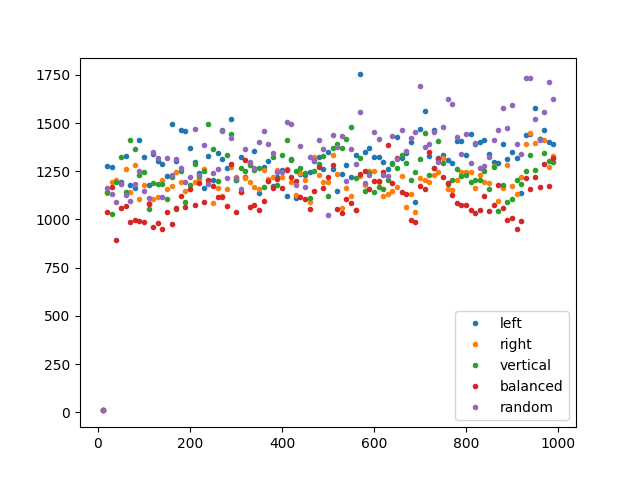
\includegraphics[width=\linewidth]{images/enc1_full.png}
    \caption{Circuit size for Bayesian net as full CPT with \texttt{ENC1} for varying vtree type and number of clauses for vtree search}
  \end{subfigure}
    \begin{subfigure}[b]{0.4\linewidth}
    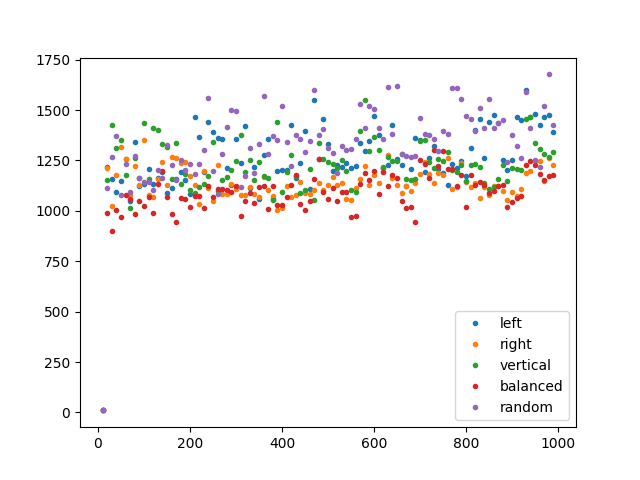
\includegraphics[width=\linewidth]{images/enc1_noisy.png}
    \caption{Circuit size for Bayesian net as noisy-OR with \texttt{ENC1} for varying vtree type and number of clauses for vtree search}
  \end{subfigure}
  \begin{subfigure}[b]{0.4\linewidth}
    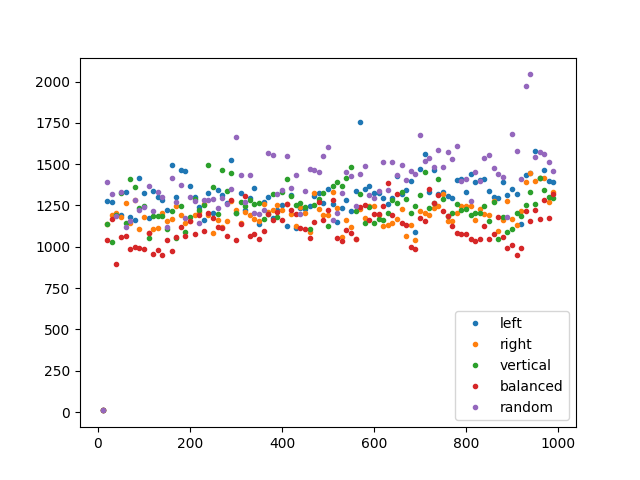
\includegraphics[width=\linewidth]{images/enc2_full.png}
    \caption{Circuit size for Bayesian net as full CPT with \texttt{ENC2} for varying vtree type and number of clauses for vtree search}
  \end{subfigure}
    \begin{subfigure}[b]{0.4\linewidth}
    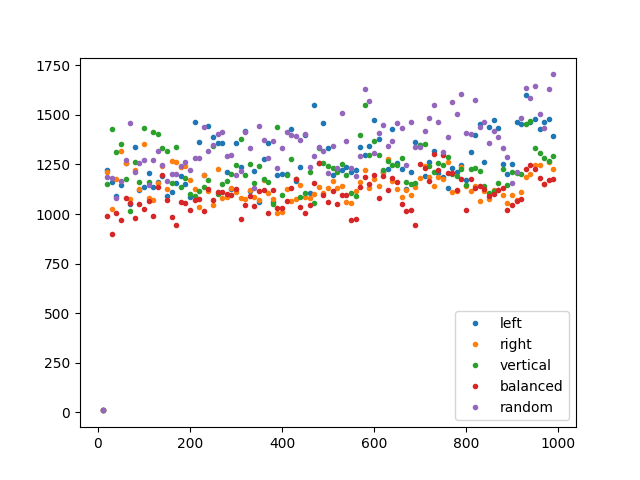
\includegraphics[width=\linewidth]{images/enc2_noisy.png}
    \caption{Circuit size for Bayesian net as noisy-OR with \texttt{ENC2} for varying vtree type and number of clauses for vtree search}
  \end{subfigure}
  \label{fig:circuits}
\end{figure}

We observe that the circuit size is overall smaller for balanced vtrees and overall greater for random vtrees. Circuit sizes for left, right and vertical vtrees usually lie between these circuit values. 

\subsubsection{Create an overview of the computational requirements of the compilation (e.g. runtime, memory)}
To create an overview of the runtime and memory usage of the python process, we used \textit{Pympler}. 

\begin{table}[h]
\centering
\begin{tabular}{l | l l}
					&	PySDD	&		Cachet	\\\hline
	Full CPT ENC1	&	1.0		&		?		\\
	Noisy OR ENC1	&	1.0		&		?		\\
	Full CPT ENC2	&	1.0000000000000004 &	?	\\
	Noisy OR ENC2	&	1.0		&		?		\\
\end{tabular}
\caption{Memory usage for \textit{PySDD} and \textit{Cachet} using \texttt{ENC1} and \texttt{ENC2}}
\label{tab:memory_pysdd_cachet}
\end{table}

\begin{table}[h]
\centering
\begin{tabular}{l | l l}
					&	PySDD	&		Cachet	\\\hline
	Full CPT ENC1	&	1.0		&		?		\\
	Noisy OR ENC1	&	1.0		&		?		\\
	Full CPT ENC2	&	1.0000000000000004 &	?	\\
	Noisy OR ENC2	&	1.0		&		?		\\
\end{tabular}
\caption{Runtime for \textit{PySDD} and \textit{Cachet} using \texttt{ENC1} and \texttt{ENC2}}
\label{tab:runtime_pysdd_cachet}
\end{table}

\subsubsection{Use WMC to compute the probabilities }
To compute the probability $P(S \mid I=\top, O = \top, R = \top)$, we add evidence to the theory $\Delta$. As mentioned by Chavria and Darwiche \cite{chavira}, there are two ways to incorporate this evidence:
\begin{enumerate}
	\item the weight associated with each indicator $\lambda_x$, whose subscript contradicts the evidence from 1 to 0.
	\item the rows that contradicts the evidence are removed from the theory being counted.
\end{enumerate}

To obtain these results, we have chosen to use the first approach. We have adapted our script which generates the \textit{PySDD} CNF file such that the $\lambda_x$ indicator variables which contradict the evidence are set to 0. However, when using this technique, we obtained results which did not match our expectations. We would expect the probability to be $99.99\%$ (see Figure \ref{fig:task_1_3_4}) but obtained a WMC of 0, which would be incorrect. We then made a script to load the \textit{PySDD} CNF file and set the weights of the literals manually. When doing this, the probabilities of the literals are $nan$.

\subsubsection{Explain briefly the main theoretical differences between the two weighted model counters.}


\begin{figure}[h]
	\centering
	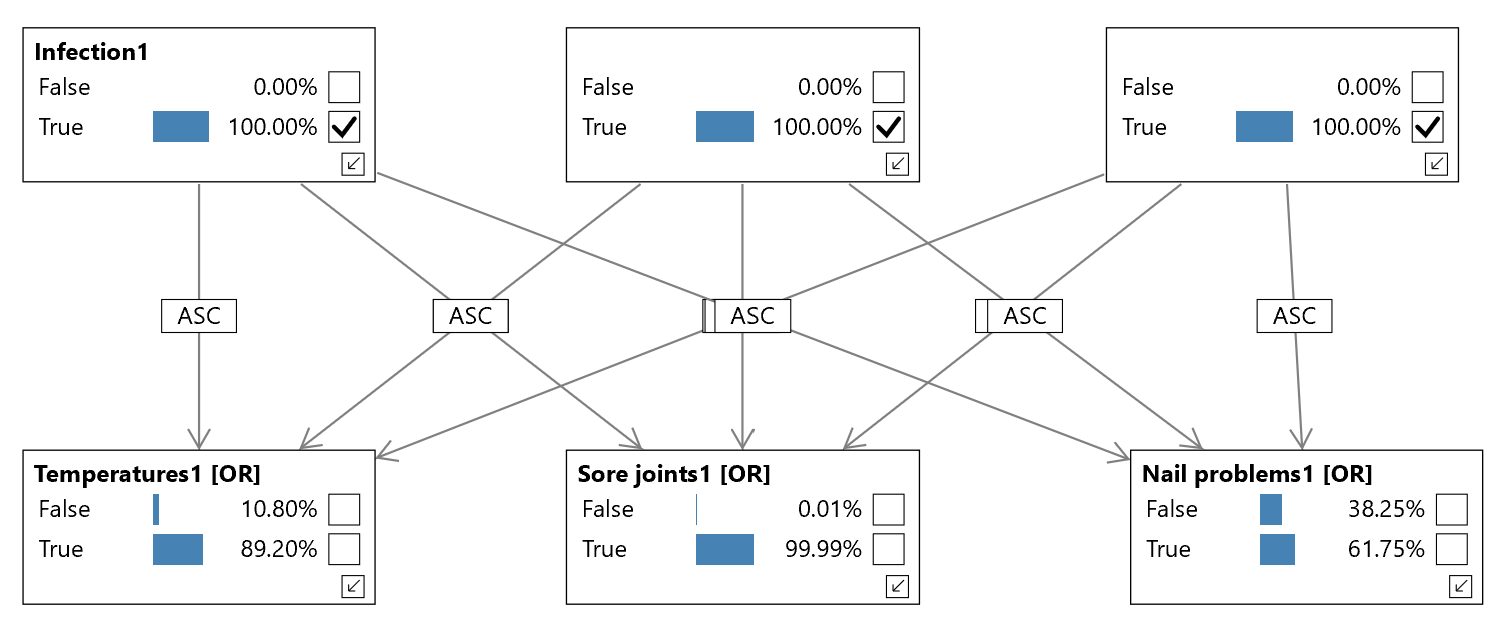
\includegraphics[width=\linewidth]{images/task_1_3_4.png}
	\caption{Probability}
	\label{fig:task_1_3_4}
\end{figure}

\section{Lifted Inference}
\section{Parameter Learning}

\newpage


\section*{Repositories}
\begin{itemize}
	\item \href{https://github.com/sventhijssen/pgmtocnf}{https://github.com/sventhijssen/pgmtocnf}
	\item \href{https://github.com/gillishermans/probabilisticprogramming_part1.2-3}{https://github.com/gillishermans/probabilisticprogramming\_part1.2-3}
	\item \href{https://github.com/sventhijssen/pysdd}{https://github.com/sventhijssen/pysdd}
\end{itemize}

\bibliography{references}
\bibliographystyle{ieeetr}

\newpage

\section*{Appendix}
\label{appendix}
\subsubsection*{Full CPTs with ENC1}
\paragraph{Variables}\mbox{}\\
\input{../out/enc1_full_enc.tex}
\newpage
\paragraph{Weights}\mbox{}\\
\input{../out/enc1_full_weights.tex}

\newpage

\subsubsection*{Noisy-ORs with ENC1}
\paragraph{Variables}\mbox{}\\
\input{../out/enc1_noisy_enc.tex}
\newpage
\paragraph{Weights}\mbox{}\\
\input{../out/enc1_noisy_weights.tex}

\newpage

\subsubsection*{Full CPTs with ENC2}
\paragraph{Variables}\mbox{}\\
\input{../out/enc2_full_enc.tex}
\newpage
\paragraph{Weights}\mbox{}\\
\input{../out/enc2_full_weights.tex}

\newpage

\subsubsection*{Noisy-ORs with ENC2}
\paragraph{Variables}\mbox{}\\
\input{../out/enc2_noisy_enc.tex}
\newpage
\paragraph{Weights}\mbox{}\\
\input{../out/enc2_noisy_weights.tex}

\end{document}
